\hypertarget{deuxiuxe8me-semaine-et-impressions-uxe0-lencre-de-chine}{%
\section{Deuxième semaine et impressions (à l'encre) de
Chine}\label{deuxiuxe8me-semaine-et-impressions-uxe0-lencre-de-chine}}

\emph{Vendredi 22 juin 2018}

Notre deuxième semaine en Chine a continué au même rythme que la
première. Nous en ressortons donc fatigués après avoir exploré les
villes de Xian, Luoyang et Nanjing.

\hypertarget{les-derniuxe8res-uxe9tapes}{%
\subsection{Les dernières étapes}\label{les-derniuxe8res-uxe9tapes}}

\begin{figure}
\centering
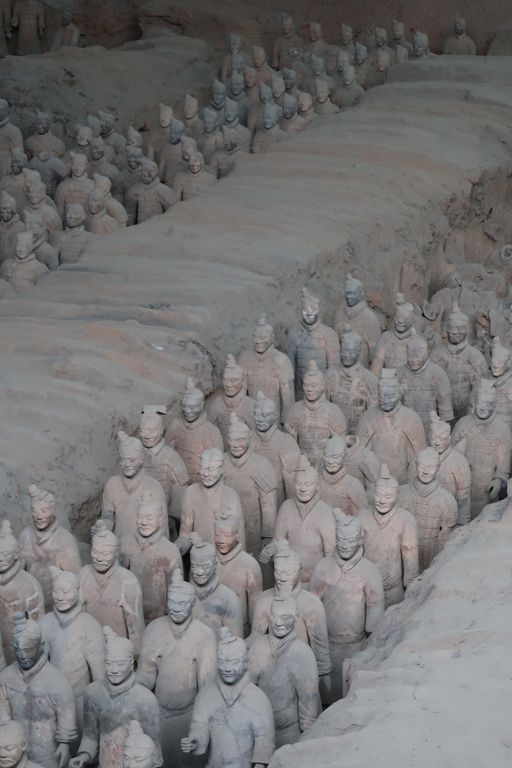
\includegraphics{images/20180622_terracotta.JPG}
\caption{Les soldats de terre cuite, rangés en ordre de bataille pour
l'au-delà.}
\end{figure}

A Xian, nous avons visité le parc des soldats de terre-cuite de
l'empereur Qin. Premier unificateur de la Chine, fervent croyant dans la
vie après la mort, il semblerait qu'il ait voulu poursuivre ses
conquêtes dans l'au-delà à l'aide d'une armée de statues de soldats, de
cavaliers, d'archers et même de généraux. Ce parc est en fait une
fouille archéologique qui continue d'évoluer depuis la découverte des
statues en 1974 (après deux millénaires passés sous terre et oubliées du
monde). Ce qui impressionne est d'abord le nombre de statues, mais aussi
le fait que chacune soit différente, avec un visage unique. L'armée est
bien fournie, avec des généraux, des chars, des cavaliers, des archers
et des fantassins. Et quand on imagine que chacune était peinte, ce
devait être incroyable ! L'affluence est tout simplement énorme. Pour
l'anecdote, le record est à 460 000 visiteurs en un jour (soit dix fois
Disneyland en régime de pointe, pour une surface visitable bien
moindre). On est à peine surpris que le sol du pavillon d'exposition est
glissant à cause de l'humidité apportée par les hordes de touristes.

A Xian, nous avons également été surpris de voir de nombreux chinois
danser dans les rues (des sortes de milongas de danse traditionnelle
chinoise), chose que nous avons revue à Luoyang. Par ailleurs, la ville
est agréable à parcourir à pied. Nous aurions aimé marcher sur ses
immenses remparts restaurés mais nous n'en avons pas eu le temps.

\begin{figure}
\centering
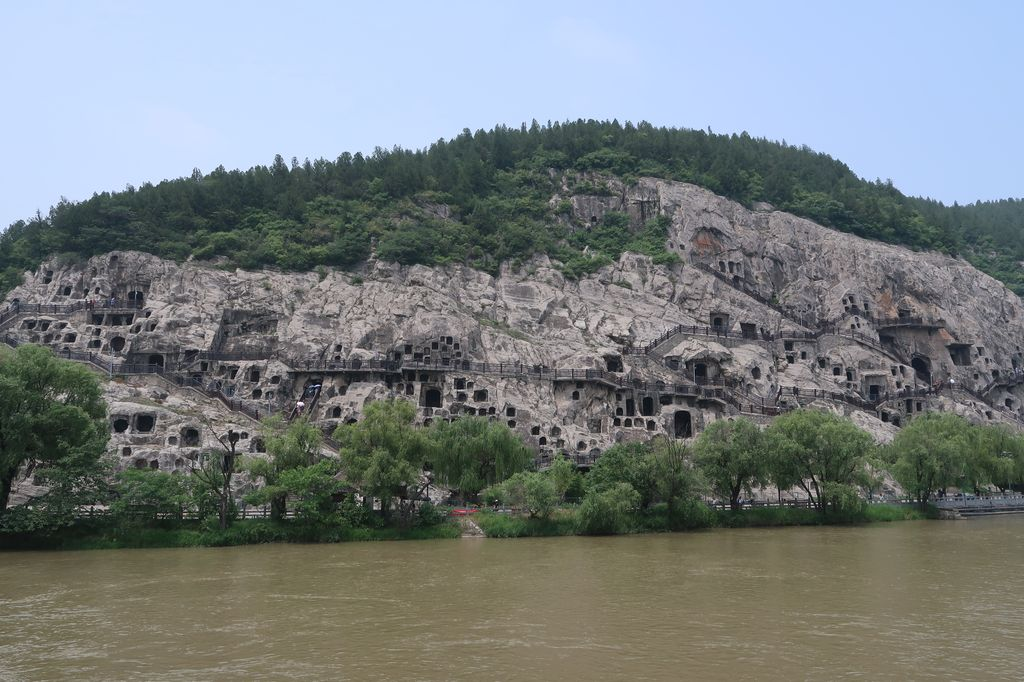
\includegraphics{images/20180622_luoyang.JPG}
\caption{Les grottes de Longmen à Luoyang. Chaque petite (ou grande)
alcôve rocheuse a accueilli une sculpture bouddhiste. Malheureusement,
la plupart a été pillée.}
\end{figure}

A Luoyang, nous avons pu explorer le très grand complexe des grottes
bouddhistes de Longmen. Des dizaines voire des centaines de milliers
d'ouvrier ont ici taillé la roche durant plusieurs centaines d'années
pour honorer la religion boudhiste.

Nous avons également visité le musée de Luoyang dans lequel nous avons
appris que la ville est célèbre pour ses pivoines (prévoir de venir au
printemps pour les admirer) depuis de nombreux siècles. Elle a également
été un point de passage important lors du commerce par la route de la
soie.

\begin{figure}
\centering
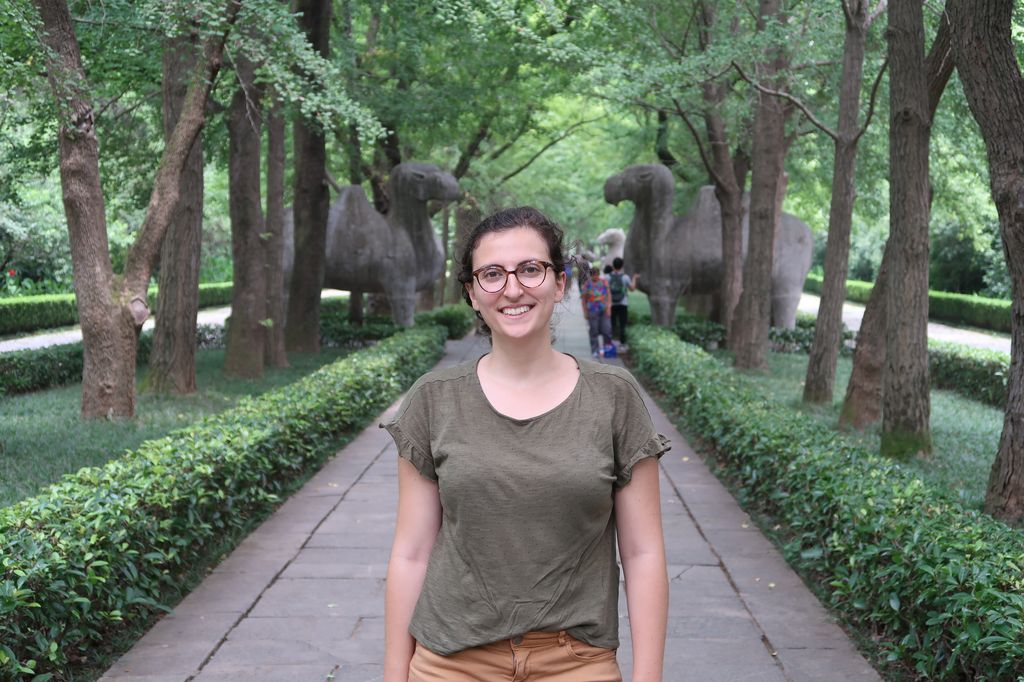
\includegraphics{images/20180622_nanjing.JPG}
\caption{Portrait dans l'allée des animaux sacrés devant la tombe Ming
de Nanjing.}
\end{figure}

Enfin, nous avons achevé de faire notre tourisme en Chine en visitant
Nanjing. On y trouve notamment, au pied de la montagne pourpre, un
sanctuaire d'un empereur de la dynastie Ming et le mémorial de Sun Yat
Sen (\emph{le} révolutionnaire chinois). Avant de quitter la ville, nous
avons visité le musée-mémorial du massacre de Nanjing, tristement
célèbre.

Voici la carte des villes que nous avons visitées lors de ces deux
dernières semaines :

\hypertarget{mapid}{}

\hypertarget{et-nos-impressions}{%
\subsection{Et nos impressions ?}\label{et-nos-impressions}}

Mais avant de quitter ce beau pays qu'est la Chine, voici quelques
observations accumulées durant les deux dernières semaines.

Et autant le dire tout de suite, nous avons été fortement impressionnés
par les choses que nous avons observées. La Chine est un pays démesuré.
Les problèmes de logistique que résolvent les villes et les
infrastructures chinoises sont plusieurs ordres de grandeur au-dessus de
ce qu'on a l'habitude de voir en région parisienne. Les transports en
sont un exemple flagrant : le nombre de lignes de métro à Beijing, la
capacité des trains, la fréquence des passages, la manière d'organiser
les trajets de foules (à l'aide de barrières métalliques), la taille des
gares ferroviaires où on a des salles d'attentes dédiées par train (et
non pas une pour tous les trains)...

\begin{figure}
\centering
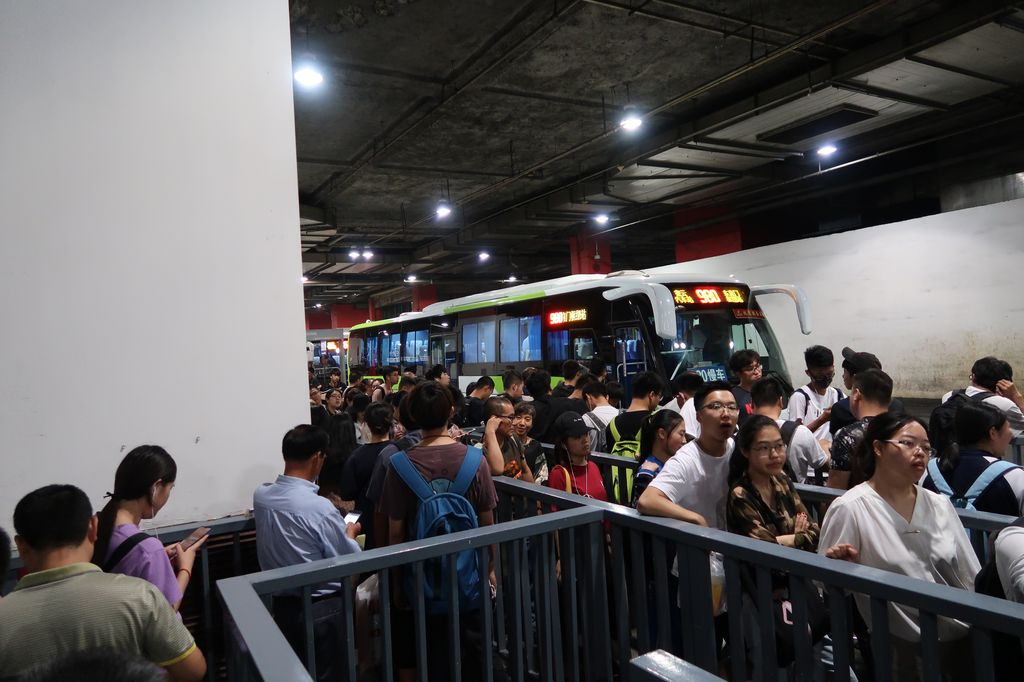
\includegraphics{images/20180622_bus.JPG}
\caption{Exemple illustratif : comment faire prendre la même ligne de
bus à 200 personnes ? 1. mettre des barrières métalliques pour guider
les gens 2. faire partir des bus toutes les cinq minutes !}
\end{figure}

Mais parlons des Chinois, que nous avons pris soin d'étudier.

Nous avons été étonnés de les voir cracher par terre (un peu partout),
fumer dans les lieux publics alors que c'est interdit, jouer des coudes
dans les transports ou dans les lieux touristiques, se tasser comme des
dingues dans le métro aux heures de pointes (à côté de ça, le RER B un
jour de grève à 8 heures du matin, c'est bon enfant), mener des
conversations téléphoniques en haut-parleur dans les transports publics.
On les croise quasiment toujours avec un thermos d'eau chaude ou de thé
à la main.En France on croise souvent des jeunes qui se baladent avec de
la musique à fond dans la rue, en Chine ce sont les personnes âgées qui
font ça, surtout dans les parcs (bon du coup c'est pas vraiment du rap
qu'ils écoutent !). On a souvent été pris en photo, parfois seulement
avec notre accord (par des adolescentes surexcitées principalement),
mais parfois plus "discrètement", si tant est que le flash à 2 mètres de
nous en pleine nuit est discret ! Même si le premier contact nous a
souvent semblé un peu froid et distant, une fois la glace brisée on a pu
échanger avec des personnes adorables et bienveillantes (un monsieur
assis à côté de nous dans le train a décidé que la barrière de la langue
ne l'empêcherait pas de nous questionner sur la France et de nous parler
de médecine traditionnelle chinoise, ce qu'il a plus ou moins réussi à
faire en jonglant avec les fonctionnalités de nos 3 téléphones
portables).

Nous avons découvert que leur nouveau Dieu s'appelle WeChat (une
application mobile un peu comme WhatsApp), qui permet de faire ses
achats en scannant le QR code du vendeur, d'afficher sa vie (comme
Facebook), de parler à ses grand-parents, de prendre le métro, de faire
des transferts d'argent, de payer le bus, d'acheter ses billets de
train, de contacter des entreprises... L'empire du milieu sous l'emprise
du smartphone ? D'après ce que nous avons vu, les transactions se font
quasiment toutes par WeChat. Lors d'une rencontre, une jeune fille nous
a même confié que ça faisait plus de six mois qu'elle n'avait pas
utilisé de l'argent papier. Si cette technologie de paiement se répand
dans le monde entier, il y a de fortes chances que les Visa et
Mastercard du futur se prénomment un jour WeChat Pay et Alipay !

\begin{figure}
\centering
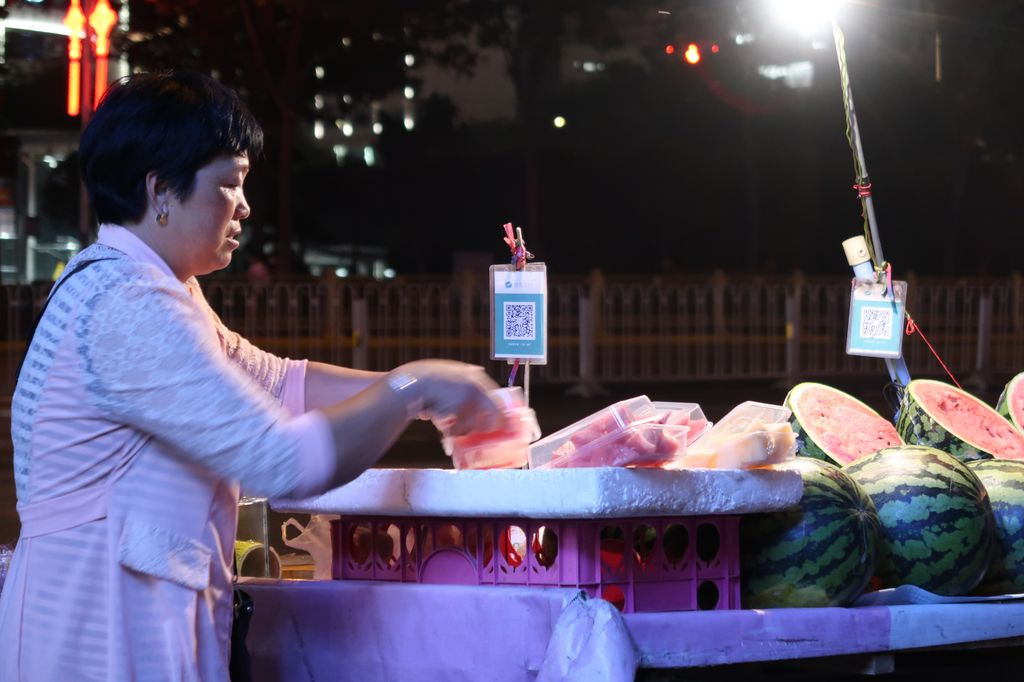
\includegraphics{images/20180622_wechat.JPG}
\caption{Puisqu'on vous dit que tout le monde utilise WeChat : même le
stand ambulant de fruits a son QR code.}
\end{figure}

Nous avons souvent eu du mal à nous faire comprendre en anglais, même
avec l'aide des applications de traduction hors-ligne. Les rares
personnes qui parlent anglais semblent souvent embêtées par nos
questions. Quelques contacts sont plus spontanés : des retraités ou bien
des enfants nous saluent par un "hello !" sympathique. Du coup pour
voyager, on s'en remet très souvent à des papiers écrits par les hôtes
des différentes auberges que nous présentons aux chauffeurs de bus ou au
passants. Mais à vrai dire, il n'y a là rien de bien curieux. Dans un
pays de 1400 millions d'habitants et donc de touristes potentiels, ce ne
sont pas les quelques millions de touristes étrangers qui comptent. Les
touristes en Chine, ce sont avant tout les chinois !

Nous avons également eu quelques tracas plus embêtants en Chine. Après
avoir visité la Cité interdite, nous avons été abordés par deux
Chinoises qui nous ont proposé de prendre un thé avec elles pour
discuter en anglais. La conversation nous a mis en confiance, mais
l'addition est salée, avec un prix plus de 20 fois supérieur à ce qui
aurait été raisonnable, que nous partageons avec elles. Très étonnés,
nous constatons sur internet que ce genre d'arnaque est arrivé à
d'autres touristes. Une autre aventure du même type concernait l'un de
nos trajets que nous devions faire en bus. Alors qu'on essayait
d'identifier notre arrêt de bus après un changement, un homme s'est
approché de nous, faisant mine de vouloir nous aider, puis nous a
affirmé que le dernier bus pour notre destination était déjà passé. Il
nous propose alors de nous emmener en voiture (c'était un trajet de 70
km) et à ce moment là, le bus est arrivé ! Belle technique de taxi pour
gagner des passagers...

Sur le plan de l'hygiène, autant dire que malgré les très nombreux
employés de nettoyage dans les rues ou devant chaque WC public, et le
nombre impressionnant de poubelles, c'est pas encore ça. On a bien
souvent vu jeter des emballages par terre sans problème. Pour les
toilettes, règle numéro 1 : amener son propre papier et savon aux
toilettes. Règle numéro 2 : travailler sa souplesse car, amateurs de
trônes confortables s'abstenir, ce sont presque toujours des toilettes à
la turque. Et deux constats étonnants : si il y a parmi les nombreuses
cabines un ou deux toilettes assis, on y trouvera des traces de
chaussures sur la cuvette. Et même s'il y a foule aux toilettes des
femmes, les cabines assises resteront inoccupées... Chez les enfants,
ceux en âge de parler ne portent plus de couches-culottes mais des
pantalons ouverts au niveau des fesses. Pourquoi ? Les parents leur font
faire leurs besoins dans les poubelles ou directement par terre sur le
trottoir !

\begin{figure}
\centering
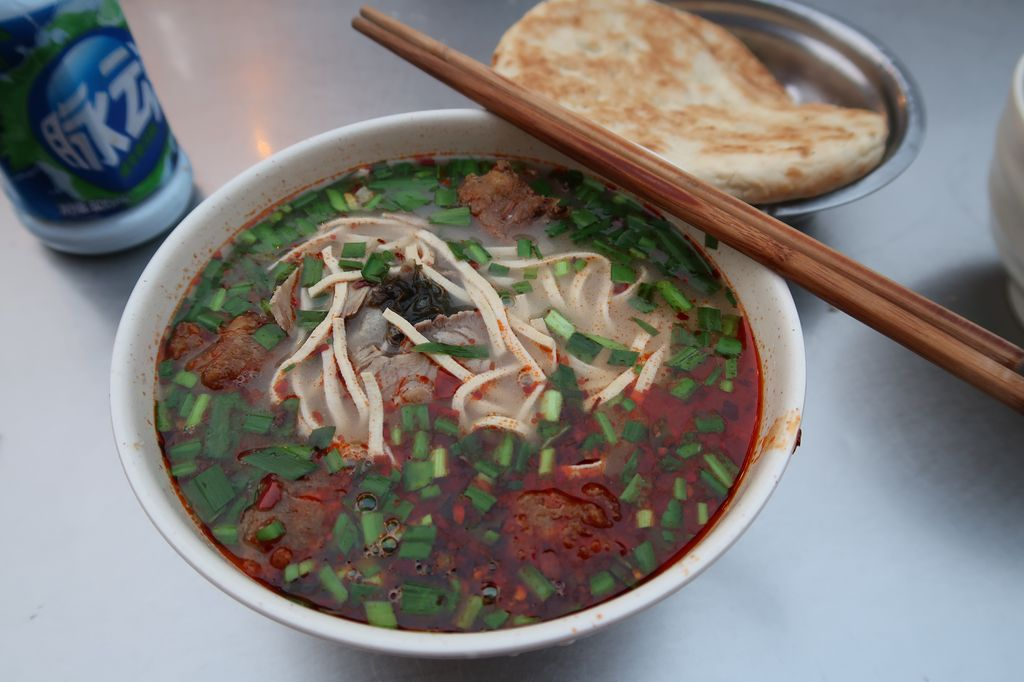
\includegraphics{images/20180622_soupe.JPG}
\caption{L'une des spécialités de Luoyang : une soupe de nouilles épicée
dans laquelle on jette des petits bouts de pain frais.}
\end{figure}

Mais concluons sur un point positif : nous avons beaucoup apprécié la
nourriture chinoise. Même en choisissant les plats au hasard, la grande
majorité de ce que nous avons pu manger était délicieux !

Un grand merci à Ruocong pour ses conseils avisés depuis Paris, et à
Longhui et Chen qui nous ont récupéré après ce tour de la Chine et aidé
à rejoindre l'aéroport.

A bientôt !

\emph{Florian et Elida}
